\documentclass [xcolor=svgnames, t] {beamer} 

\ifdefined\hyperref 
\usepackage[utf8]{inputenc}
\usepackage{booktabs, comment} 
\usepackage[absolute, overlay]{textpos} 
\useoutertheme{infolines} 
\setbeamercolor{title in head/foot}{bg=internationalorange}
\setbeamercolor{author in head/foot}{bg=dodgerblue}
\usepackage{csquotes}
\usepackage[style=verbose-ibid,backend=bibtex]{biblatex}
\bibliography{bibfile}
\usepackage{amsmath}
\usepackage[makeroom]{cancel}
\usepackage{multicol}
\usepackage{nameref}
\usepackage{textpos}

\usetheme{Madrid}
\definecolor{myuniversity}{RGB}{0, 60, 113}
\definecolor{internationalorange}{RGB}{231, 93,  42}
 	\definecolor{dodgerblue}{RGB}{0, 119,202}
\usecolortheme[named=myuniversity]{structure}
\usepackage{tikz}


\title[GAN and SVM to identify candidates to RG]{One-class SVM to identify candidates to Reference Genes based on the augment of RNA-seq data with Generative Adversarial Networks}

\author[Edwin J. Rueda]{\textbf{Edwin J. Rueda}\inst{1} \hspace{1pt} Rommel Ramos\inst{1} \\ Edian F. Franco\inst{1} \hspace{1pt} Orlando Belo\inst{2} \hspace{1pt} Jefferson Morais\inst{1}}

\institute[UFPA]{
\normalsize
\inst{1} Federal University of Pará, Belém, Brazil\\[1pt]
\inst{2} University of Minho, Braga, Portugal\\[1pt]
\vspace{22pt}
The International Conference on Computational Science and its Aplications (ICCSA) 2020}
%\titlegraphic{\includegraphics[height=2cm]{figures/logo_ufpa.eps}


\begin{document}
\begin{frame}
 \titlepage   
\end{frame}

%################################################
%---------------- SUMMARY -----------------
%################################################
\begin{frame}{Summary}
\vspace{1cm}
\begin{center}
   \begin{itemize}
     \item Introduction
     \vspace{.5cm}
     \item Proposed Method
     \vspace{.5cm}
     \item Experiments and Results
     \vspace{.5cm}
     \item Conclusions and Future Works
 \end{itemize} 
\end{center}
 
\end{frame}

%################################################
%---------------- INTRODUCTION -----------------
%################################################
\begin{frame}{Introduction}
\begin{center}
\begin{itemize}
    \item \textbf{Reference Genes (RG)} 
    \begin{itemize}
        \item Constitutive genes
        \vspace{3pt}
        \item Expressed in all cells
        \vspace{3pt}
        \item Used in internal controls (gene expression analysis)
    \end{itemize}
\end{itemize}
\vspace{5pt}

\includegraphics[scale=.3]{figures/rt_pcr.eps}
%Reference gene must in turn demonstrate the variability resulting from imperfections of the technology used and preparatory procedures—this ensures that any variation in the amount of genetic material will relate to the same extent as the object of research and control.
%para normalizar la expresión génica
%-Los genes de referencia en Quantitative RT-PCR sirven para normalizar los datos, debido a que los GR tienen un minimo cambio de su expresión genética en diferentes condiciones de estrés. El gen de referencia a su vez debe demostrar la variabilidad resultante de las imperfecciones de la tecnología utilizada y los procedimientos preparatorios, esto asegura que cualquier variación en la cantidad de material genético se relacione en la misma medida que el objeto de investigación y el de control (gen de referencia).
\begin{itemize}
    \item Normalize gene expression
    \item Demonstrates the variability and imperfections of the technology
\end{itemize}

\end{center}
\end{frame}

%#################################################
%----------------- Second frame ------------------
%#################################################
%Based on optimziation algorithms: minimum cost network flow problem
\begin{frame}{Introduction}
\Large\textcolor{dodgerblue}{\textbf{Identify candidates for Reference Genes}}
\vspace{5pt}
\begin{center}
\begin{itemize}
    \normalsize
    \item Pipeline:
\end{itemize}
\vspace{13pt}
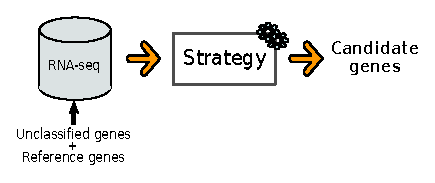
\includegraphics[scale=1.3]{figures/strategy.eps}
\vspace{18pt}
\begin{itemize}
    \normalsize
    \item Strategies
    \begin{itemize}
        \item Based on clustering (Euclidean distance)
        \vspace{3pt}
        \item Based on optimization algorithms
\end{itemize}
\end{itemize}
\end{center}
\end{frame}


%################################################
%---------------- PROPOSED METHOD ---------------
%################################################
%#####################################################
%------------------ PROPOSED METHOD ------------------
%#####################################################
\begin{frame}{Proposed Method}
\begin{center}

\begin{itemize}
    \item Steps:
      \begin{enumerate}
        \vspace{3pt}
        \item Generative Adversarial Networks to augment of RNA-seq data
        \vspace{3pt}
        \item One-Class SVM to select candidate genes
      \end{enumerate} 
\end{itemize}
\vspace{20pt}
\includegraphics[scale=.8]{figures/methodology_iccsa.eps}
\vspace{10pt}
\begin{itemize}
    \item Initial step: data processing
\end{itemize}
\end{center}
\end{frame}

%#####################################################
%------------------ DATA PROCESSING ------------------
%#####################################################
\begin{frame}{Proposed Method}
\Large\textcolor{dodgerblue}{\textbf{Data processing}}
    \begin{center}
        \normalsize
    \begin{multicols}{2}[\columnsep2em] 
    \vspace{5pt}
    \begin{itemize}
            \item Pipeline:
            \vspace{3pt}
            \begin{enumerate}
                \item Normalization with RPKM
                \begin{equation*}
                    RPKM = \frac{numReads*10^9}{geneLength*TMReads}
                \end{equation*}
                \item $\log_{2}+1$
                \vspace{2pt}
                \item Remove outliers based on the Coefficient of Variation
                \begin{equation*}
                    CV = \frac{\sigma}{\mu}
                \end{equation*}
                \item Data scaled between $[-1, 1]$
            \end{enumerate}
        \end{itemize}
    \columnbreak
    \includegraphics[scale=1.2]{figures/data_processing.eps}
    \end{multicols}
    \end{center}
\end{frame}
%#####################################################
%------------ GENERATIVE ADVERSARIAL NETS ------------
%#####################################################
\begin{frame}{Proposed Method}
    \Large\textcolor{dodgerblue}{\textbf{Generative Adversarial Networks (GAN)}}
    \normalsize
    \vspace{5pt}
    \begin{itemize}
        \item Steps:
        \vspace{3pt}
        \begin{enumerate}
            \item Training the Discriminator network and freezing their weights
            \vspace{3pt}
            \begin{figure}
                \centering
                  \includegraphics[scale=.8]{figures/training_step_1.eps}
            \end{figure}
            \item Training the Generator network
            \vspace{3pt}
            \begin{figure}
                \centering
                \includegraphics[scale=.8]{figures/training_step_2.eps}
            \end{figure}
        \end{enumerate}
    \end{itemize}

\end{frame}
%#####################################################
%------------ GENERATIVE ADVERSARIAL NETS ------------
%#####################################################
\begin{frame}{Proposed Method}
    \Large\textcolor{dodgerblue}{\textbf{Proposed architecture}}
    \normalsize
    \vspace{2pt}
    \begin{columns}
    \column{.5\textwidth}
    \begin{itemize}
        \item Generator network
        \vspace{5pt}
        \begin{figure}
            \centering
            \includegraphics[scale=2]{figures/generator_network.eps}
        \end{figure}
    \end{itemize}
    
    \column{.5\textwidth}
    \begin{itemize}
        \item Discriminator network
        \vspace{5pt}
        \begin{figure}
            \centering
            \includegraphics[scale=2]{figures/discrimanotr_network.eps}
        \end{figure}
    \end{itemize}
    \end{columns}
    \vspace{12pt}
    \begin{itemize}
        \item A Normal distribution $N(0,1)$ as a noise vector
        \item Stochastic Gradient Descent to compute the gradients
    \end{itemize}
\end{frame}

%#####################################################
%----------------- GAN EVALUATION ------------------------
%#####################################################
\begin{frame}{Proposed Method}
    \Large\textcolor{dodgerblue}{\textbf{Evaluation}}
    \normalsize
    \vspace{5pt}
    \begin{itemize}
        \item A proposed Similarity metric $S(x, x')$ to evaluate the performance of the GAN:
        \begin{equation*}
            S\left(x,x'\right)=\sum_{i}^{m}\sum_{j}^{n_{g}}\sum_{k}^{n_{f}} \frac{|{x_{i}^{(k)}-{x'}_{j}^{(k)}}|}{n_{f}n_{g}m}  + |0.5 - \frac{1}{n_{g}}\sum_{j}^{n_{g}}\hat{y}_j|
        \end{equation*}
        \item $\hat{y}$: Class predicted by $D$ network for a synthetic gene
        \vspace{1pt}
        \item $x'$: Set of synthetic genes generated by the $G$ network
        \vspace{1pt}
        \item $x$: Set of Reference Genes
        \vspace{1pt}
        \item $m=0$: Number of Reference Genes
        \vspace{1pt}
        \item $n_g=300$: Number of synthetic genes
        \vspace{1pt}
        \item $n_f=9$: Number of features (gene expression)
    \end{itemize}
\end{frame}

\begin{frame}{Proposed Method}
    \Large\textcolor{dodgerblue}{\textbf{Evaluation}}
    \normalsize
    \vspace{7pt}
    \begin{itemize}
        \item A proposed $E(x')$ metric to select the best sample of synthetic data:
        \vspace{8pt}
        \Large
        \begin{equation*}
            E(x') = \frac{1}{n_{g}}\sum_{j}^{n_{g}}\left[CV({x'}_{j}) + \frac{1-D({x'}_{j})}{D({x'}_{j})}\right]
        \end{equation*}
        \normalsize
        \vspace{4pt}
        \item $CV$: Coefficient of variation
        \vspace{1pt}
        \item $x'$: Set of synthetic genes generated by the $G$ network
        \vspace{1pt}
        \item $n_g=300$: Number of synthetic genes
        \vspace{1pt}
        \item \textbf{Other metrics:} Binary Cross-Entropy, Precision score
    \end{itemize}
\end{frame}

%#####################################################
%----------------- ONE-CLASS SVM ---------------------
%#####################################################
\begin{frame}{Proposed Method}
    \Large\textcolor{dodgerblue}{\textbf{One-Class SVM}}
    \normalsize
    \vspace{5pt}
    \begin{itemize}
        \item Based on novelty detection
    \end{itemize}
    \vspace{-9pt}
    \begin{columns}
    \column{.49\textwidth}
    \begin{itemize}
        \item Decision boundary
        \vspace{2pt}
        \begin{figure}
            \centering
            \includegraphics[scale=.5]{figures/svm_boundary.eps}
        \end{figure}
    \end{itemize}
    \column{.48\textwidth}
    \begin{itemize}
        \item Novelty detection
        \vspace{2pt}
        \begin{figure}
            \centering
            \includegraphics[scale=.5]{figures/svm_classifier.eps}
        \end{figure}
    \end{itemize}
    \end{columns}
    \vspace{5pt}
    \begin{itemize}
        \item Implements the RBF kernel (Gaussian kernel)
        \begin{equation*}
        k \left(x,y\right)=e^{-\gamma\lVert{x-y}\rVert^2}
        \end{equation*}
    \end{itemize}
\end{frame}

%#####################################################
%-------------- ONE-CLASS SVM EVALUATION -------------
%#####################################################
\begin{frame}{Proposed Method}
    \Large\textcolor{dodgerblue}{\textbf{Evaluation}}
    \normalsize
    \vspace{7pt}
    \begin{itemize}
        \item Recall score to evaluate the performance of the One-Class SVM
        \vspace{8pt}
    \end{itemize}
    \Large
    \begin{equation*}
        Recall = \frac{TP}{TP + FN}
    \end{equation*}
    \begin{itemize}
        \normalsize
        \vspace{4pt}
        \item $TP$: True Positives
        \vspace{2pt}
        \item $FN$: False Negatives
        \vspace{2pt}
        \item Recall score allows to measure the ability of the classifier to find all positive samples (RG)
        \vspace{2pt}
        \item A recall score close to one indicates that the classifier has a good performance
    \end{itemize}
\end{frame}

%################################################
%------------ EXPERIMENTS AND RESULTS -----------
%################################################
\begin{frame}{Experiments and Results}
    
\end{frame}

\begin{frame}{Governing equations (Mean flow)\autocite{Lecture3}}
  
 \textit{\textbf{RANS} equations for incompressible flow}:\\
  \textbf{Continuity equation}
  
     \begin{equation}
      \frac{\partial \overline{u_{i}}}{\partial x_{i}}=0
  \end{equation} 
  
 
  
  
  \textbf{Momentum equations }
  \begin{equation}
      \frac{\partial \overline{u_{i}} }{\partial t} + \overline{u_{j}} \frac{\partial \overline{u_{i}} }{\partial x_{j}} = -\frac{1}{\rho}\frac{\partial \overline{P}}{\partial x_{i}}+\nu\frac{\partial ^2\overline{u_{i}}}{\partial x_{j}\partial x_{j}}-\frac{\partial \overline{u_{i}'u_{j}'}}{\partial x_{j}}+\overline{g_{i}}
  \end{equation}
  
   \textbf{Scaler equation }
  \begin{equation}
     \frac{\partial \overline{\phi}}{\partial t}+\overline{u_{i}}\frac{\partial \overline{\phi}}{\partial x_{i}}=\frac{\partial}{\partial x_{i}}(D\frac{\partial \overline{\phi}}{\partial x_{i}})-\frac{\partial (\overline{{u_{i}^{'}\phi^{'}}})}{\partial x_{i}}
  \end{equation}
  
  
\end{frame}


%################################################
%---------------- THANK YOU ---------------
%################################################
\begin{frame}
\author{}
\institute{
	\fontsize{34pt}{34pt}\selectfont
	\textcolor{blue!50!black}{\bf Thank you!}\\[12pt]
	}
\date{
	\normalsize
	Edwin J. Rueda (edwin.rojas@icen.ufpa.br)\\[1pt]
	Federal University of Pará (UFPA)\\[1pt]
	Belém, Pará, Brazil\\
	}
\titlepage
\end{frame}


\end{document}